\chapter{Skalierbarkeit und Wartbarkeit}

In diesem Kapitel wird der Begriff \textit{Skalierbarkeit} erklärt sowie die notwendigen Kompromisse erläutert, die bei der Entwicklung einer verteilten skalierbaren Anwendung eingegangen werden müssen. Das \textbf{CAP-}Theorem beschreibt die Grenzen eines verteilen Systems und \textbf{BASE} fasst größtmögliche Anforderungen an ein verteiltes System zusammen. Danach werden die \textit{Best Practices} und \textit{Patterns} beschrieben, deren Einhaltung die Entwicklung einer modulären Webanwendung mit austauschbaren Komponenten ermöglicht. 

\subsection{\colorbox{green}{Skalierbarkeit}}\label{scale}
%\section{Skalierbarkeit}\label{scale}

Der Begriff \textit{Skalierbarkeit} beschreibt die Fähigkeit eines Systems, das bei wachsenden Anforderungen, entweder die Leistung der vorhandenen Ressourcen verbessert oder zusätzlich die neuen Ressourcen hinzufügt.

\colorbox{red}{Der Begriff \textit{Skalierbarkeit} beschreibt die Fähigkeit eines Systems, aufgrund der wachsenden Anforderungen, entweder die Leistung der vorhandenen Ressourcen zu verbessern oder zusätzlich die neuen Ressourcen hinzufügen.}

Das System, bei dem die neuen Ressourcen hinzugefügt werden, nennt man \textit{verteilte Systeme}.

Bei der Skalierung sind zwei Arten zu unterscheiden, eine \textit{vertikale} und eine \textit{horizontale Skalierung}, die demnächst näher erläutert wird.

%\subsection{Vertikale Skalierbarkeit}
\subsection{\colorbox{green}{Vertikale Skalierbarkeit}}

Die \textit{vertikale Skalierbarkeit (scale-up)} strebt eine qualitative Steigerung der Leistungsfähigkeit an, bei der die bereits eingesetzten Ressourcen, beispielsweise durch die Speichererweiterung oder CPU-Steigerung, verbessert werden.

Die vertikale Skalierbarkeit hat den Vorteil, dass die Daten nicht verteilt werden müssen. Die Nebenläufigkeit kann mit \textit{Threads} realisiert werden. Jedoch hat die vertikale Skalierbarkeit ihre Grenzen - ein Rechner kann nicht endlos vergrößert werden. 

%\subsection{Horizontale Skalierbarkeit}
\subsection{\colorbox{green}{Horizontale Skalierbarkeit}}

Im Gegensatz zur vertikalen Skalierung verteilt die \textit{horizontale Skalierbarkeit (scale-out)} die Daten auf verschiedenen Knoten im großen Cluster, wobei die quantitative Steigerung der Leistungsfähigkeit angestrebt wird. Somit können mehrere weniger leistungsfähige, nicht so teuere Rechner eingesetzt werden. %Dadurch ist es möglich, sehr große horizontale Skalierbarkeit zu gewährleisten, da die Knoten somit nicht so stark, im Vergleich zur vertikalen Skalierung überlastet sind. 
Ein verteiltes System kann viel mehr als ein vertikales Skalieren - Erweiterung eines Clusters um weitere Rechner ist sehr einfach und Clusters können auch sehr groß werden. Die horizontale Skalierbarkeit ist günstiger - je leistungsfähiger ist der Rechner, desto teuerer ist seine Erweiterung. Allerdings unterscheidet sich die Entwicklung eines verteilten Systems von den klassischen Anwendungen, die auf einer Maschine laufen, da die Daten in dem Cluster verteilt sind. Die \textit{Trade-offs} einer verteilten Anwendung wurden bereits in der CAP-Theorem \textbf{(Kap. \ref{cap})}  formalisiert.

%\subsection{ACID-Prinzip}\label{acid}
\subsection{\colorbox{red}{ACID-Prinzip}}\label{acid}

Des Weiteren sind sinnvolle Regeln zum effektiven und effizienten Umgang mit Transaktionen unvermeidbar. Solche Regeln sind in einem \acid\ definiert.

\textbf{ACID} steht für \Acid, \aCid, \acId\ und \aciD\ und beschreibt somit die Eigenschaften eines Datenbankmanagementsystems zur Sicherung der Datenkonsistenz bei Transaktionen.
\begin{itemize}

\item \Acid: Die \textit{Atomarität} einer Transaktion bedeutet, dass sie entweder ganz oder gar nicht ausgeführt wird. Falls eine Transaktion abgebrochen wird, werden alle im Laufe der Transaktion schon durchgeführte Änderungen rückgängig gemacht, um Konflikte mit der Ausführung neuer Transaktionen zu vermeiden.%was eigentlich zu einer sicheren Fehlerisolierung führt.
\item \aCid: Die \textit{Konsistenz} besagt, dass vor und auch nach dem Ablauf einer Transaktion die Integrität und Plausibilität der Datenbestände gewährleistet werden. Die Integrität der Datenbank ist es möglich, beispielsweise mit Integritätsbedingungen\footnote{Unter Integritätsbedingungen (Zusicherungen, Assertions) sind Bedingungen zu verstehen, die die Korrektheit der gespeicherten Daten sichern. Diese werden in SQL zum Beispiel mithilfe von CONSTRAINTS formuliert. Folgende CONSTRAINTS sind möglich: NULL, NOT NULL, PRIMARY KEY, FOREIGN KEY etc.} zu gewährleisten. 
%Diese werden bis zur abgeschlossenen Transaktion in einem konsistenten Zustand gehalten und werden bei der Transaktion in einen anderen konsistenten Zustand überführt.
\item \acId: Die \textit{Isolation} dient zu Kapselung von Transaktionen, um unerwünschte Nebenwirkungen vermeiden zu können. Die Transaktionen müssen unabhängig voneinander ablaufen.
\item \aciD: Die \textit{Dauerhaftigkeit} gewährleistet nach einer erfolgreichen Transaktion die Persistenz aller Datenänderungen. Im Falle eines Systemfehlers oder Neustarts müssen die Daten nichtsdestotrotz zur Verfügung stehen, dass sie in einer Datenbank dauerhaft gesichert sein müssen.
%dauerhaft in der Datenbank zu erhalten.
%Genauer gesagt, die Daten müssen dauerhaft auf einem Datenträger gesichert sein
\end{itemize}

%\subsection{Das CAP-Theorem}\label{cap}
\subsection{\colorbox{green}{Das CAP-Theorem}}\label{cap}

Im Jahr 2000 präsentierte Eric A. Brewer das \textbf{CAP}-Theorem - ein Ergebnis seiner Forschungen zu verteilten Systemen. Das Ergebnis zeigte, dass bei den verteilten Systemen alle drei folgenden Anforderungen wie \Cap, \cAp\ und \caP\ gleichzeitig nicht zu erfüllen sind.
%\colorbox{yellow}{Im Jahr 2000} hielt Brewer\footnote{Eric A. Brewer ist ein Informatik-Professor an der University of California, Berkeley und einer der Erfinder der Suchmaschine Inktomi} die Keynote auf dem ACM Symposium on Principles of Distributed Computing (PODC)\footnote{PODC2000: \url{http://www.podc.org/podc2000/}, zugegriffen am 02.01.2017}, einer Konferenz über die Grundlagen der Datenverarbeitung in verteilten Systemen\footnote{In einem verteilten System im Bereich Datenverarbeitung werden gespeicherte Daten mehrfach über mindestens zwei verschiedene Server repliziert und miteinander synchronisiert, um die Verfügbarkeit der Daten zu erhöhen und die Zugriffszeiten der User zu verringern.} (Principles of Distributed Computing).  In seiner Keynote stellte Brewer sein \textbf{CAP}-Theorem vor, ein Ergebnis seiner Forschungen zu verteilten Systemen an der University of California \cite[S. 13]{Kurowski.2012}. Brewer's Theorem wurde im Jahr 2002 von Seth Gilbert und Nancy Lynch formal bewiesen.
\begin{figure}[H]
\centering
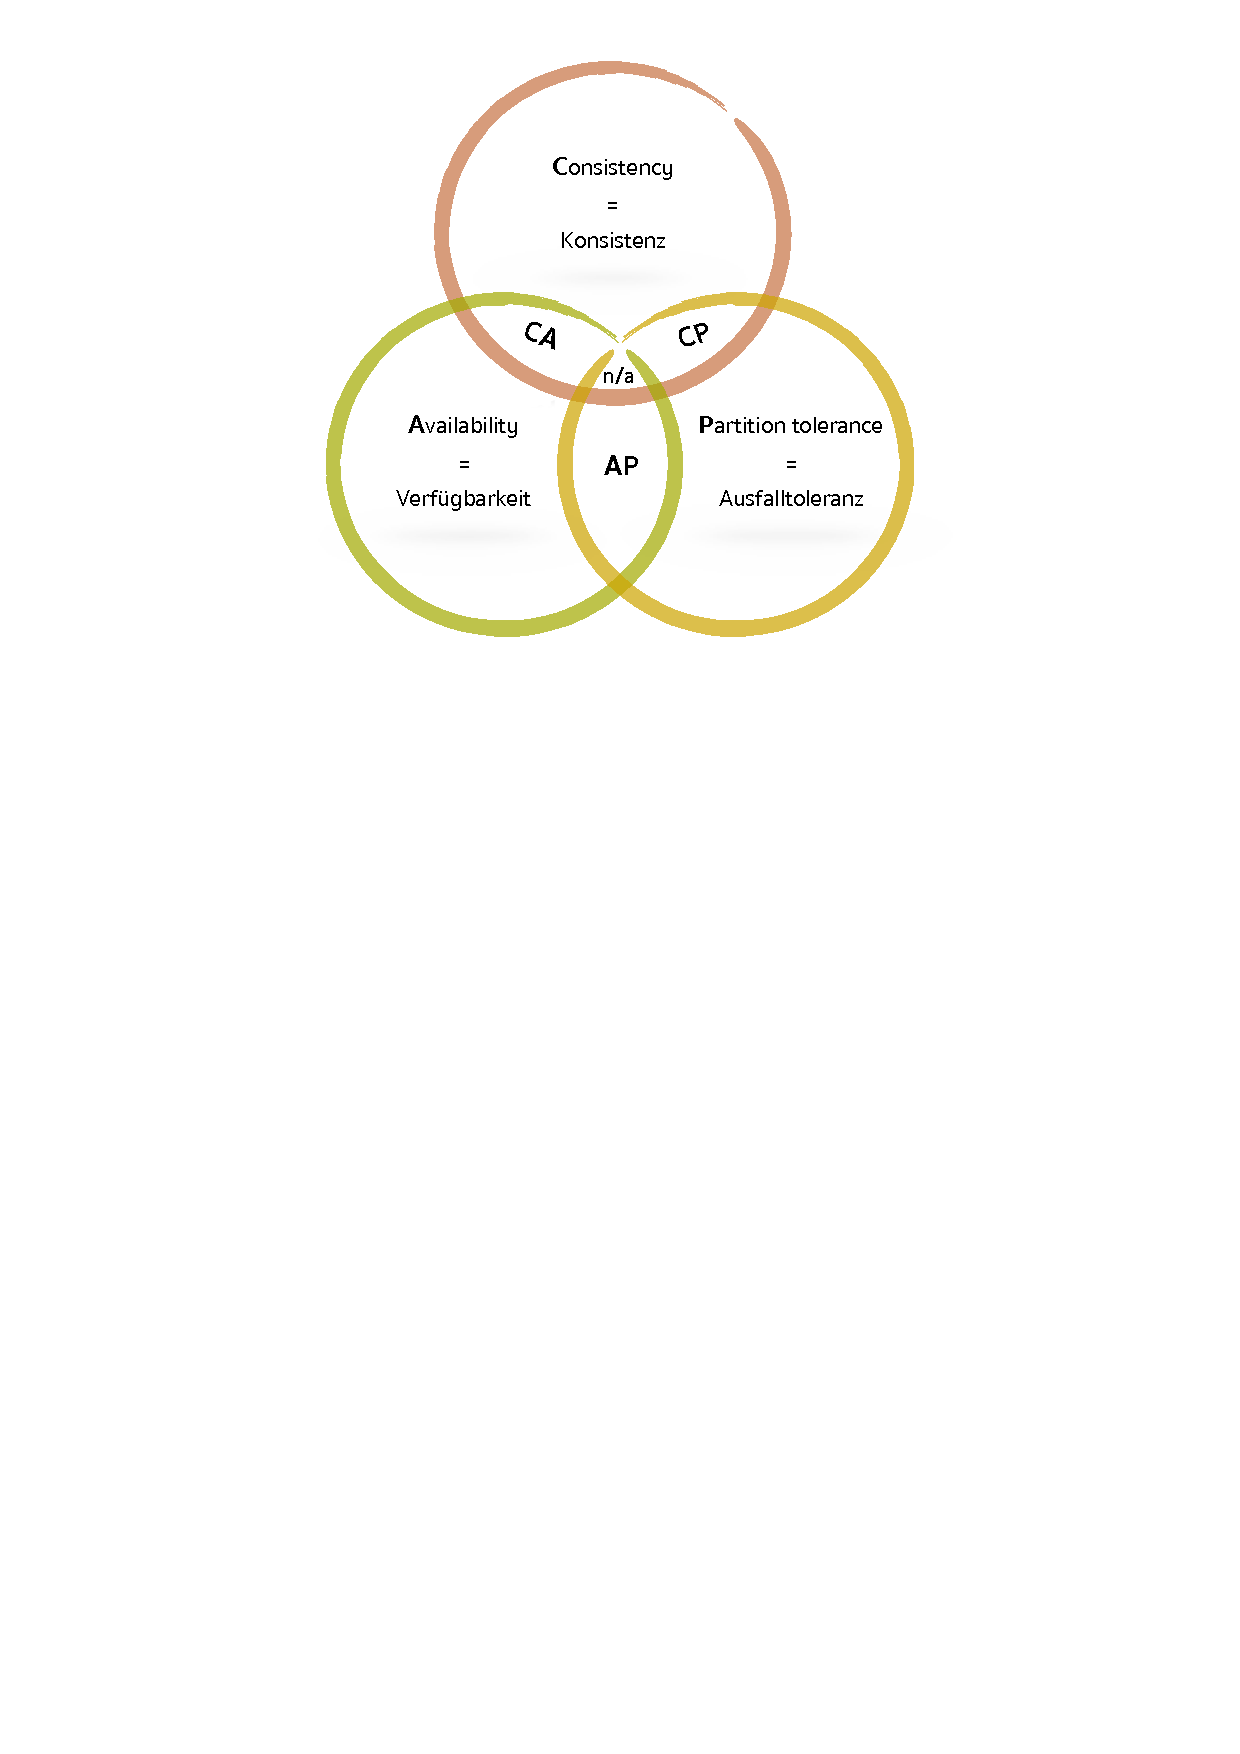
\includegraphics[trim = 0mm 189mm 0mm 9mm, clip, width=1.0\textwidth]{resources/myPictureForCAP}
\caption[\textbf{CAP}-Theorem]{Anforderungen an verteilte Systeme gemäß dem \textbf{CAP}-Theorem}
\label{img:cap}
\end{figure}

Das Akronym \textbf{CAP} steht für die englischsprachigen Begriffe  \Cap, \cAp\ und \caP. Diese sind mögliche Anforderungen an eine verteilte Anwendung.
\begin{itemize}
\item \Cap: Diese Anforderung ist erfüllt, wenn nach Abschluss einer atomaren\footnote{Eine atomare Transaktion bedeutet, dass sie entweder ganz oder gar nicht ausgeführt wird. Falls eine atomare Transaktion abgebrochen wird, werden alle im Laufe der Transaktion bereits durchgeführte Änderungen rückgängig gemacht.} Transaktion (oder Interaktion mit dem System) nicht nur die manipulierenden Datensätze, sondern auch alle replizierenden Knoten in einem großen Cluster über die gleichen Daten verfügen. Wenn ein Wert auf einem Knoten geändert wird und die Interaktion mit dem System abgeschlossen wird, muss der aktualisierte Wert von anderen Knoten zurückgeliefert werden können. Dies hat zur Folge, dass ein System erst dann die Interaktion abschließen darf, wenn sichergestellt ist, dass die Änderungen auf alle Datenkopien angewendet wurden. Für die verteilten Systeme, die Daten replizieren, resultiert es in langen Antwortzeiten für die Schreiboperationen.

\item \cAp: Die \textit{Hochverfügbarkeit} ist eine weitere Anforderung, die besagt, dass immer alle gesendeten Anfragen durch User an das System mit einer akzeptablen Reaktionszeit beantwortet werden müssen.

\item \caP: Die \textit{Partitions- oder Ausfalltoleranz} bedeutet, dass der Ausfall eines Knoten bzw. eines Servers aus einem Cluster das verteilte System nicht beeinträchtigt und es weiterhin fehlerfrei funktioniert. Falls einzelne Knoten in so einem System ausfallen, wird deren Ausfall mit den verbleibenden Knoten aus dem Cluster kompensiert, um die Funktionsfähigkeit des Gesamtsystems aufrecht zu halten.

\end{itemize}

Die graphische Darstellung für das Brewer's \textbf{CAP}-Theorem ist aus der Abbildung \ref{img:cap} zu entnehmen. Wie die Abbildung \ref{img:cap} erkennen lässt, können in einem verteilten System gleichzeitig und vollständig nur zwei von drei Anforderungen  \Cap, \cAp, \caP\ erfüllt werden. Konkret aus der Praxis bedeutet das, dass es für eine hohe Verfügbarkeit und Partitions- oder Ausfalltoleranz notwendig ist, die Anforderungen an die Konsistenz zu lockern \cite[S. 31]{Edlich.2011}.

Die Anforderungen in Paaren klassifizieren gemäß dem \textbf{CAP}-Theorem bestimmte Datenbanktechnologien. Für jede Webanwendung muss daher individuell entschieden werden, ob sie als ein \textbf{CA-}, \textbf{CP-} oder \textbf{AP-}System zu realisieren ist.
\begin{itemize}
\item \textbf{CA} (\textbf{C}onsistency und \textbf{A}vailability): Die klassischen relationalen Datenbankmanagementsysteme (RDBMS) wie Oracle, DB2 etc. fallen in \textbf{CA}-Kategorie, die vor allem auf  \Cap\ und \cAp\ aller Knoten in einem Cluster hinzielen. Hierbei werden die Daten nach dem \textbf{ACID}-Prinzip verwaltet. Die relationalen Datenbanken sind für Ein-Server-Hardware konzipiert und vertikal skalierbar. Das bedeutet, dass solche Systeme mit hochverfügbaren Servern betrieben werden und \caP\  nicht unbedingt in Frage kommt.

%\begin{itemize}
%\item keine Partitionstoleranz
%\item (Relationale) Datenbank ermöglicht verteilte Transaktionen zur Konsistenzwahrung
%\item Voraussetzung: funktionierendes Netzwerk (kein Nachrichtenverlust)
%\item URL: \url{http://dbs.uni-leipzig.de/file/NoSQL_SS14_01_Intro.pdf}
%\end{itemize}

\item \textbf{CP} (\textbf{C}onsistency und \textbf{P}artition tolerance): Ein gutes Beispiel für die Webanwendungen, die zu der \textbf{CP-}Kategorie zuzuordnen sind, sind Banking-Anwendungen. Für solche Anwendungen ist es wichtig, dass die Transaktionen zuverlässig durchgeführt werden und der mögliche Ausfall eines Knotens verschmerzt werden kann. 
%
%\begin{itemize}
%\item keine Verfügbarkeit
%\item im Falle von Netzwerkpartitionierung werden Transaktionen blockiert
%\item Vermeidung möglicher Konflikte bei Merge, dadurch Sicherstellung der Konsistenz
%\item URL: \url{http://dbs.uni-leipzig.de/file/NoSQL_SS14_01_Intro.pdf}
%\end{itemize}

\item \textbf{AP} (\textbf{A}vailability und \textbf{P}artition tolerance): Für die Anwendungen, die in die \textbf{AP-}Kategorie fallen, rückt die Anforderung \Cap\ in den Hintergrund. Beispiele für solche Anwendungen sind die Social-Media-Sites wie Twitter oder Facebook, da die Hauptidee der Anwendung nicht verfällt, wenn zum gleichen Zeitpunkt die replizierten Knoten nicht die gleiche Datenstruktur aufweisen. 
\end{itemize}
%
%\begin{itemize}
%\item keine Konsistenz
%\item Writes stets möglich auch wenn keine Kommunikation mit anderen Knoten möglich
%(z.B. Synchronisation)
%\item Notwendigkeit der Auflösung inkonsistenter Daten, d.h. verschiedene Versionen des
%selben Datums an verschiedenen Knoten
%\item URL: \url{http://dbs.uni-leipzig.de/file/NoSQL_SS14_01_Intro.pdf}
%\end{itemize}



%\subsection{BASE}\label{base}
\subsection{\colorbox{yellow}{BASE}}\label{base}

\textbf{BASE} steht für \BAse, \baSe, \basE\ und beschreibt den Gegenteil zu den strengen \textbf{ACID}-Kriterien \textbf{(Kap. \ref{acid})}. \textbf{BASE} ist wie \textbf{CAP}-Theorem \textbf{(Kap. \ref{cap})} auch für verteilte Datenbanksysteme formuliert, für die die \textit{Konsistenz} nicht mehr im Vordergrund steht, sondern die \textit{Verfügbarkeit} eines Systems. Bei solchen Systemen, die nach dem \textbf{BASE}-Prinzip gestaltet sind, ist eher wichtig, dass für alle Clients das System ständig verfügbar ist. Die Clients müssen nicht unbedingt zu dem gleichen Zeitpunkt die gleichen Daten sehen.


%\section{Wartbarkeit}\label{maintenance}
\section{\colorbox{yellow}{Wartbarkeit}}\label{maintenance}

Um die Wartungs- und Erweiterungsfähigkeiten von der Software zu gewährleisten, sollen die grundlegenden Designprinzipien eingehalten werden. \textbf{SOLID}\footnote{SOLID, \url{https://web.archive.org/web/20150906155800/http://www.objectmentor.com/resources/articles/Principles_and_Patterns.pdf}, zugegriffen am 03.02.2017}, beschrieben von Martin Fowler, steht für fünf Prinzipien des objektorientierten Designs. Die richtige Anwendung dieser Prinzipien bringt die Struktur in das Softwareprodukt. Die Software wird mit der Einhaltung von \textbf{SOLID} Regeln entwickelt, bestehend aus vielen kleinen Modulen. Jedes Modul hat eine klare Funktion und die Interaktion zwischen den Modulen erfolgt über explizit definierte Schnittstellen. Im Einzelnen beschreibt \textbf{SOLID} folgende Regeln:

\begin{itemize}

\item \textit{Single responsibility principle} - Eine Klasse (oder Modul) soll nur eine bestimmte Funktion abdecken und eine Funktion soll von einer Klasse implementiert werden. Martin Fowler betont, dass für die Änderung einer Klasse nur ein Grund geben kann. Im Kontext der Prototypanwendung könnte das Backend Teil beispielsweise zwei Funktionen haben, die Bearbeitung von Frontend-Anfragen und Verwaltung der Daten in der Datenbank. Es wäre schlechtes Design, wenn eine Klasse beide diese Funktionalitäten implementieren würde. Es gäbe dann mehrere Gründe für die Änderung dieser Klasse - z. B. Änderung in Kommunikation mit Frontend oder in der Datenhaltung.

\item \textit{Open/closed principle} - Die Klassen/Module sollen für die Erweiterung offen sein, die bestehenden Klassen sollen aber nicht geändert werden. Die Idee dahinter ist, dass wenn die neuen Funktionalitäten eingeführt werden, darf der bestehende Code nur minimal geändert werden. Zum Beispiel die Daten der Foto-Verwaltungs-Anwendung wurden bisher in der relationalen Datenbank gehalten und zusätzlich soll die Datenhaltung in der NoSQL Datenbank implementiert werden. Die NoSQL Datenhaltung soll in eigenem Modul implementiert werden und darf die Codebasis für die Interaktion mit relationaler Datenbank nicht ändern. 

\item \textit{Liskov substitution principle} - Die Subklassen dürfen das Verhalten der Elternklassen nicht ändern. Der Code, der auf bestehenden Funktionen der Elternklassen aufgebaut ist, muss auch mit Subklassen fehlerfrei funktionieren.

Wenn z. B. die Foto-Verwaltungs-Anwendung erweitert wird und z. B. die Videos verwaltet werden müssen, wäre es falsch die Klasse \textit{`Video`} aus der Klasse \textit{`Foto`} abzuleiten, weil Videos andere Eigenschaften als Bilder haben.

\item \textit{Interface-segregation principle} - Die Interfaces sollen so klein wie möglich sein und nur einzelne Funktionen abdecken.

\item \textit{Dependency inversion principle} - Die Abhängigkeiten zwischen Modulen sollen über Abstraktionen \textit{(Interfaces)} gekoppelt werden. Ein Modul soll keine direkte Abhängigkeit zu den anderen Modulen haben, die Abhängigkeiten werden zu den Interfaces definiert. Demzufolge können die Module die Interfaces implementieren und ohne großen Aufwand ausgetauscht werden. Die implementierende Module sehen nur die Interfaces, die zu implementieren sind und wissen nicht bei welchen Modulen diese eingesetzt werden. Wir nehmen Backend der Foto-Verwaltungs-Anwendung nochmal als Beispiel und betrachten die Interaktion zwischen dem \textit{Service} Modul, der mit Frontend interagiert und dem Modul der Daten in der relationalen Datenbank verwaltet. Anstatt eine Referenz zu diesem spezifischen Datenbankmodul zu deklarieren, wird eine Referenz zu einem Interface deklariert, der die Datenhaltungskomponente beschreibt. Aus der Sicht von dem \textit{Service} Modul gibt es eine Menge von notwendigen Operationen, um die Daten zu speichern oder abzurufen. Diese Operationen sind ähnlich für verschiedene Arten von Datenhaltung und deswegen werden die in einem \textit{Interface} zusammengefasst. Der Service Modul deklariert eine Abhängigkeit zu diesem Interface. Dieser Interface kann von verschiedenen Datehaltungskomponenten implementiert werden.

\end{itemize}

%\subsection{Dependency Injection (DI)}\label{di}
\subsection{\colorbox{yellow}{Dependency Injection (DI)}}\label{di}

\textit{Dependency Injection} ist der nächste Schritt nach \textit{Dependency Inversion}. Der \textit{Dependency Injection Pattern} basiert auf dem \textit{Inversion of Control Konzept}. Das bedeutet, dass die verwendeten Klassen sich nicht mehr selbst um Ablauf und Abhängigkeiten kümmern, sondern diese werden an eine externe Komponente ausgelagert. Die Klasse gibt sozusagen die Kontrolle ab und lässt sich von außen steuern. Konkret bedeutet es, dass die Klassen nur die Abhängigkeiten zu den Interfaces deklarieren müssen und die konkrete Implementierung wird zur Laufzeit eingefügt (injected). Die genauere Zusammensetzung einer Applikation wird deklarativ definiert, es können auch verschiedene Konfigurationen existieren.

---------------------
\colorbox{red}{ist der untere Teil unbrauchbar?????}
---------------------

Ein weiteres Ziel, dass in dieser Abschlussarbeit verfolgt wird, ist es unter anderem, eine Architektur nicht nur für eine skalierbare, sondern auch für eine wartbare Webanwendung aufzustellen. Für die ordentliche Wartbarkeit der Anwendung sind die Grundlagen für das \di\ Pattern\footnote{Inversion of Control Containers and the Dependency Injection pattern, \url{https://martinfowler.com/articles/injection.html}, zugegriffen am 03.02.2017} unvermeidbar. Das Prinzip \di\ wird bei vielen Frameworks wie zum Beispiel Google Guice\footnote{Google Guice, \url{https://github.com/google/guice}, zugegriffen am 03.02.2017}, Dragger\footnote{Dager, \url{http://square.github.io/dagger/}, zugegriffen am 03.02.2017} etc. umgesetzt. Im Kapitel `Implementierung` \textbf{(Kap. \ref{implement})} wird das Prinzip \di\ sowohl im Präsentationsschicht durch JavaScript-Framework \textbf{Angular 2} als auch im Logiksschicht durch \textbf{Spring Framework} veranschaulicht.

Der Einsatz des \di\ Pattern ermöglicht den Entwicklern, der Arbeitsaufwand für die Entwicklung großer Anwendungen stark zu reduzieren. Bei seinem Einsatz wird eine \textbf{lose Kopplung} der Anwendungskomponenten erreicht, die dem Entwickler die Konzentration auf die Entwicklung einzelner Komponenten unabhängig voneinander ermöglicht. Die Unabhängigkeit der Programmteile erleichtert dem Entwickler nicht nur die Anwendungskomponenten unabhängig voneinander zu entwicklen, sondern auch diese leichter zu testen. 

%\subsubsection{Inversion of Control (IoC)}
\subsubsection{\colorbox{red}{Inversion of Control (IoC)}}

Eine wichtige Idee hinter dem \textit{Dependency Injection Pattern} entspringt dem \textit{Inversion of Control} Konzept. Das bedeutet, dass die verwendeten Klassen sich nicht mehr selbst um Ablauf und Abhängigkeiten kümmern, sondern dass dies eines der Frameworks, wie z. B. \textbf{Spring} \textbf{(Kap. \ref{spring})} , übernimmt. Die Klasse gibt sozusagen die Kontrolle ab und lässt sich von außen steuern. Dadurch wird eine \textbf{lose Kopplung} von Abhängigkeiten erreicht. Das ist der zentrale Vorteil der \textit{DI}.

%\subsubsection{Dependency Injection und Mock-Objekte}
\subsubsection{\colorbox{red}{Dependency Injection und Mock-Objekte}}\label{di}

Enge Kopplung von Abhängigkeiten erschwert nicht nur die Erweiterung oder Änderung von Codebasis, sondern auch die Testbarkeit. Zum Beispiel mit UnitTests sollen die Komponenten unabhängig von den anderen Komponenten getestet werden. Dafür werden die Abhängigkeiten zu anderen Komponenten simuliert. Falls die zu testende Methode die Daten aus der Datenbank für Ihre Berechnung benötigt, kann die Datenbankverbindung simuliert und die Testdaten zurückgegeben werden. Solche Klassen, die die Abhängigkeiten simulieren nennt man \textbf{Mock-Klassen}.

Die lose Kopplung des \textit{DI} Patterns ermöglicht die Verwendung von Mock-Objekten. Die entsprechenden Abhängigkeiten werden zur Laufzeit von Tests von dem entsprechenden Framework injiziert, somit sind seitens des Entwicklers keine weiteren Schritte notwendig.
---------------------

---------------------
%\subsection{MVC-Pattern}\label{mvc}
\subsection{\colorbox{yellow}{MVC-Pattern}}\label{mvc}

\textbf{MVC}\footnote{Objektorientierte Programmierung, \url{http://openbook.rheinwerk-verlag.de/oop/oop_kapitel_08_002.htm}, zugegriffen am 20.01.2017} ist ein Prinzip der modernen Programmierung und ist nach wie vor das wichtigste und verbreitetste Muster für die Architektur von objektorientierten Anwendungen. Heutzutage ist Model-View-Controller ein bekanntes Model, das in vielen Programmiersprachen für die Architektur von Frameworks und Anwendungen verwendet wird.

Das Ziel des \textbf{MVC}-Musters ist Geschäftslogik einer Anwendung von der Benutzerschnittstelle abzutrennen, so dass Entwickler einen Bereich bequem verändern kann und der Rest der Anwendung wird dadurch nicht beeinflusst.
Es soll ein flexibler Programmierentwurf geben, der eine spätere Änderung oder Erweiterung erleichtert und eine Wiederverwendbarkeit und Austauschbarkeit einzelner Komponenten ermöglicht.

%\subsubsection{Workflow}
\subsubsection{\colorbox{yellow}{Workflow}}

Der Workflow-Prozess \textbf{(Abb. \ref{img:mvc})} stellt eine vollständige Beschreibung aller Aktivitäten, der \textbf{MVC}-Pattern voraussetzt. Die Abbildung \ref{img:mvc} ist grober Workflow des \textbf{MVC}-Pattern anhand einer Beispielinteraktion und ihrer Ergebnisses präsentiert.
\begin{figure}[H]
\centering
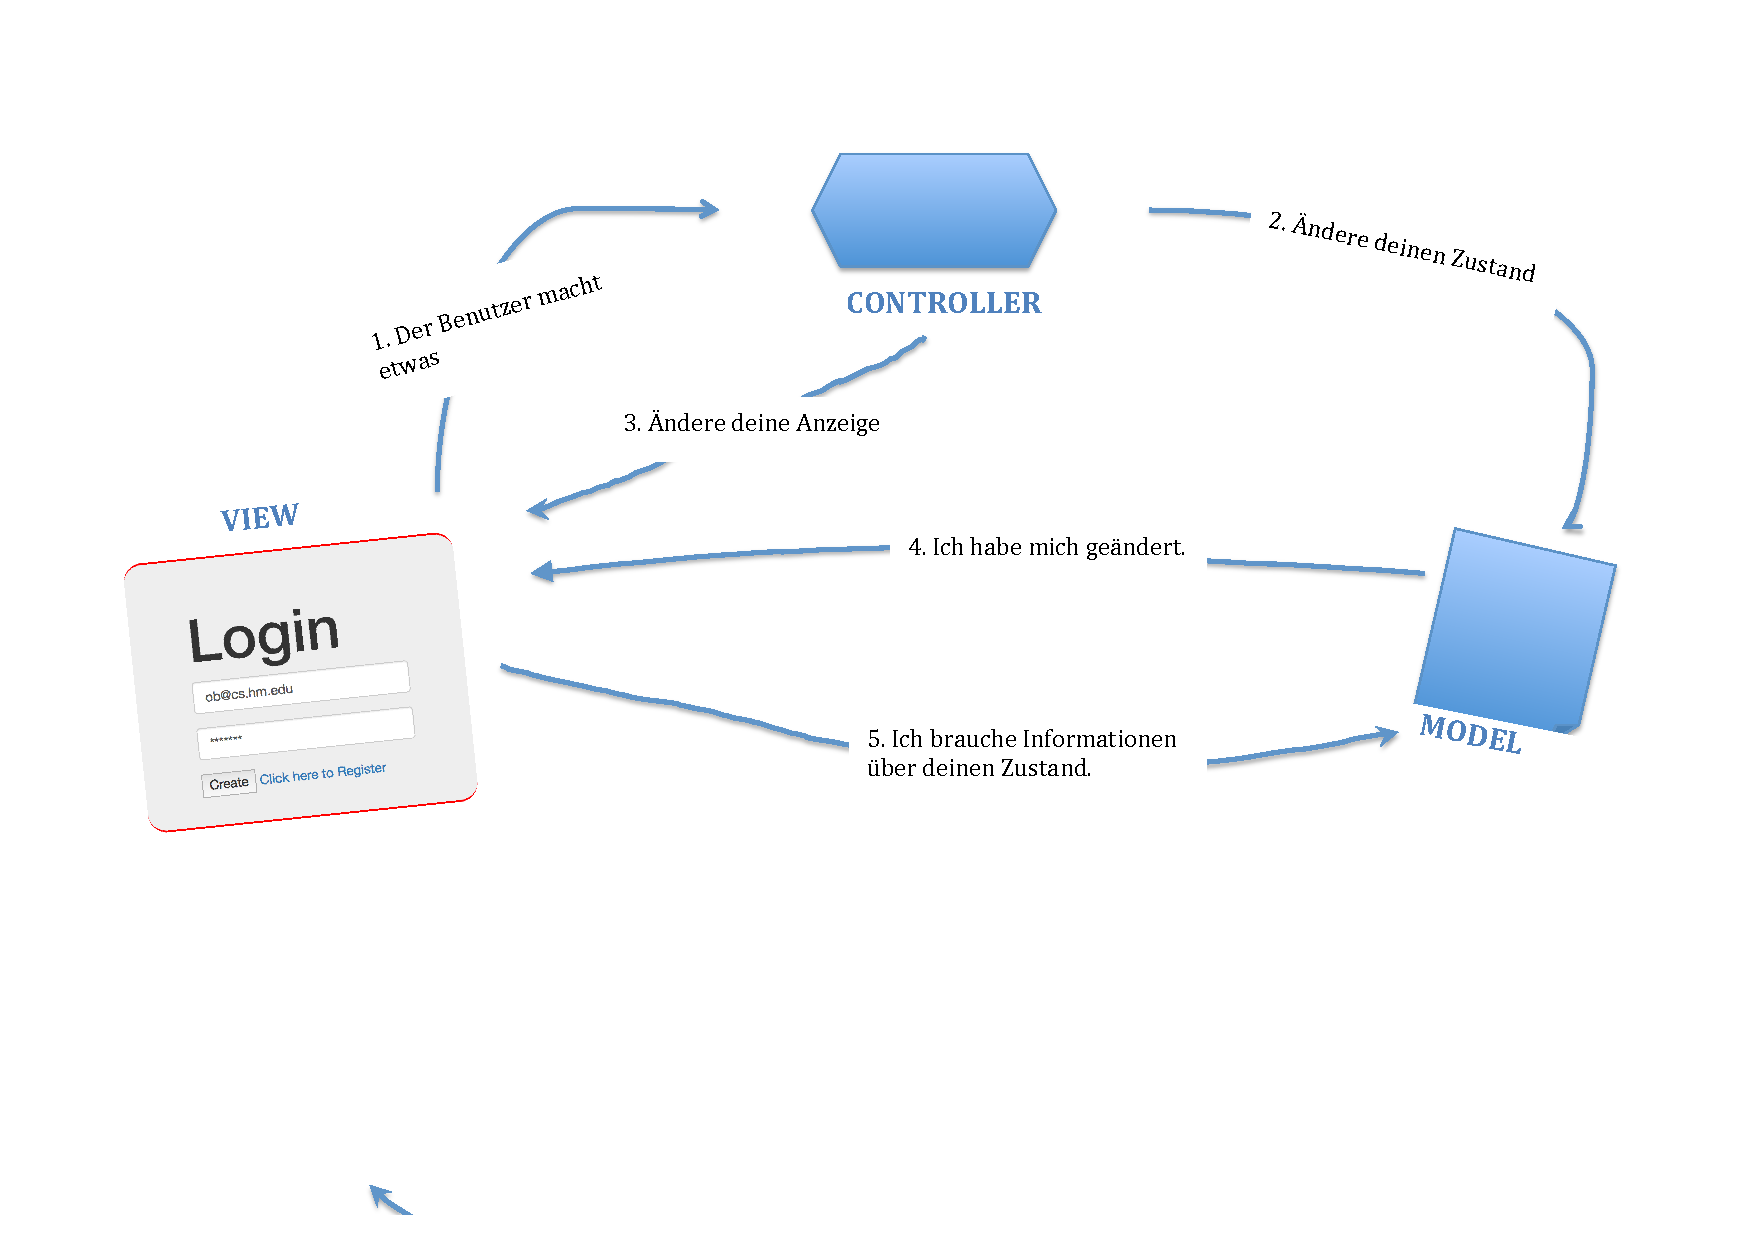
\includegraphics[trim = 0mm 60mm 0mm 20mm, clip, width=1.0\textwidth]{resources/mvc}
\caption[Workflow zum MVC-Konzept]{Workflow zum MVC-Konzept}
\label{img:mvc}
\end{figure}

\textbf{Beschreibung des Workflow-Prozesses:}
\begin{enumerate}
\item \textbf{Der Benutzer interagiert mit dem View}\\
Der Benutzer führt irgendeine Aktion an dem View aus. Dadurch teilt der View dem Controller mit, was zu tun ist. Erst dann ist die Aufgabe des Controllers. entsprechende Steuerungsmaßnahmen zu ergreifen.

\item  \textbf{Der Controller fordert das Model auf, seinen Zustand zu ändern}\\
Nach der Ausführung irgendeiner Aktion an dem View durch den Benutzer, nimmt der Controller die Aktion an und interpretiert sie. Bei der Interpretation stellt der Controller heraus, was gemacht werden muss und wie das Model aufgrund dieser Aktion beeinflusst werden kann.

\item  \textbf{Der Controller kann auch den View auffordern, seinen Zustand zu ändern}\\
Der Controller kann bei der Ausführung einer Aktion auch den View auffordern, sich zu ändern. Zum Beispiel, beim Klick auf einen Button durch den Benutzer kann der gerade eingeblendete View ausgeblendet und ein anderer View eingeblendet werden.

\item  \textbf{Das Model informiert den View über seine Zustandsänderung}\\
Dem Model selbst sind Views und Controller nicht bekannt bzw. diese sind an dem Model nicht festprogrammiert. Aber das Model kann diejenige, die sich beim Model registriert haben, über seine Zustandsänderungen informieren, \textbf{(Kap. \ref{observer})}.

\item  \textbf{Der View erfragt den Zustand des Models}\\
Das Model stellt weitere Methoden zur Verfügung, über die der aktuelle Zustand des Models erfragen werden kann. 
Jeder View kann sich somit durch den Aufruf dieser Methoden über den Zustand des Models informieren.

\end{enumerate}
Um die Benachrichtigung über Modelsänderungen an Views oder auch an Controller zu ermöglichen, nutzt MVC das sogenannte Beobachter Muster \textbf{(Kap. \ref{observer})}.

%\subsubsection{Beobachter Muster}\label{observer}
\subsubsection{\colorbox{yellow}{Beobachter Muster}}\label{observer}

Beobachter Muster (engl. Observer-Pattern) ist eines der am meisten genutzten und bekanntesten Pattern. In diesem Muster teilt die Komponente Model allen Interessenten proaktiv mit, dass ihr Zustand geändert wurde.

Würde man ohne das \textbf{Observer}-Pattern eine solche Beobachtung implementieren, so müssten die Interessenten die Komponente Model regelmäßig abfragen, ob ihr Zustand geändert wurde.
%\paragraph{Idee}
\paragraph{\colorbox{yellow}{Idee}}
Beim \textbf{Observer}-Pattern gibt es eine Komponente (Observable), deren Zustand sich ändern kann und andere Komponenten (Observers), die über Zustandsänderung informiert werden sollten. Das \textbf{Observer}-Pattern sieht vor, dass die Observers sich beim Observable registrieren und bei einer Zustandsänderung informiert Observable alle registrierte Objekte.

\begin{figure}[H]
\centering
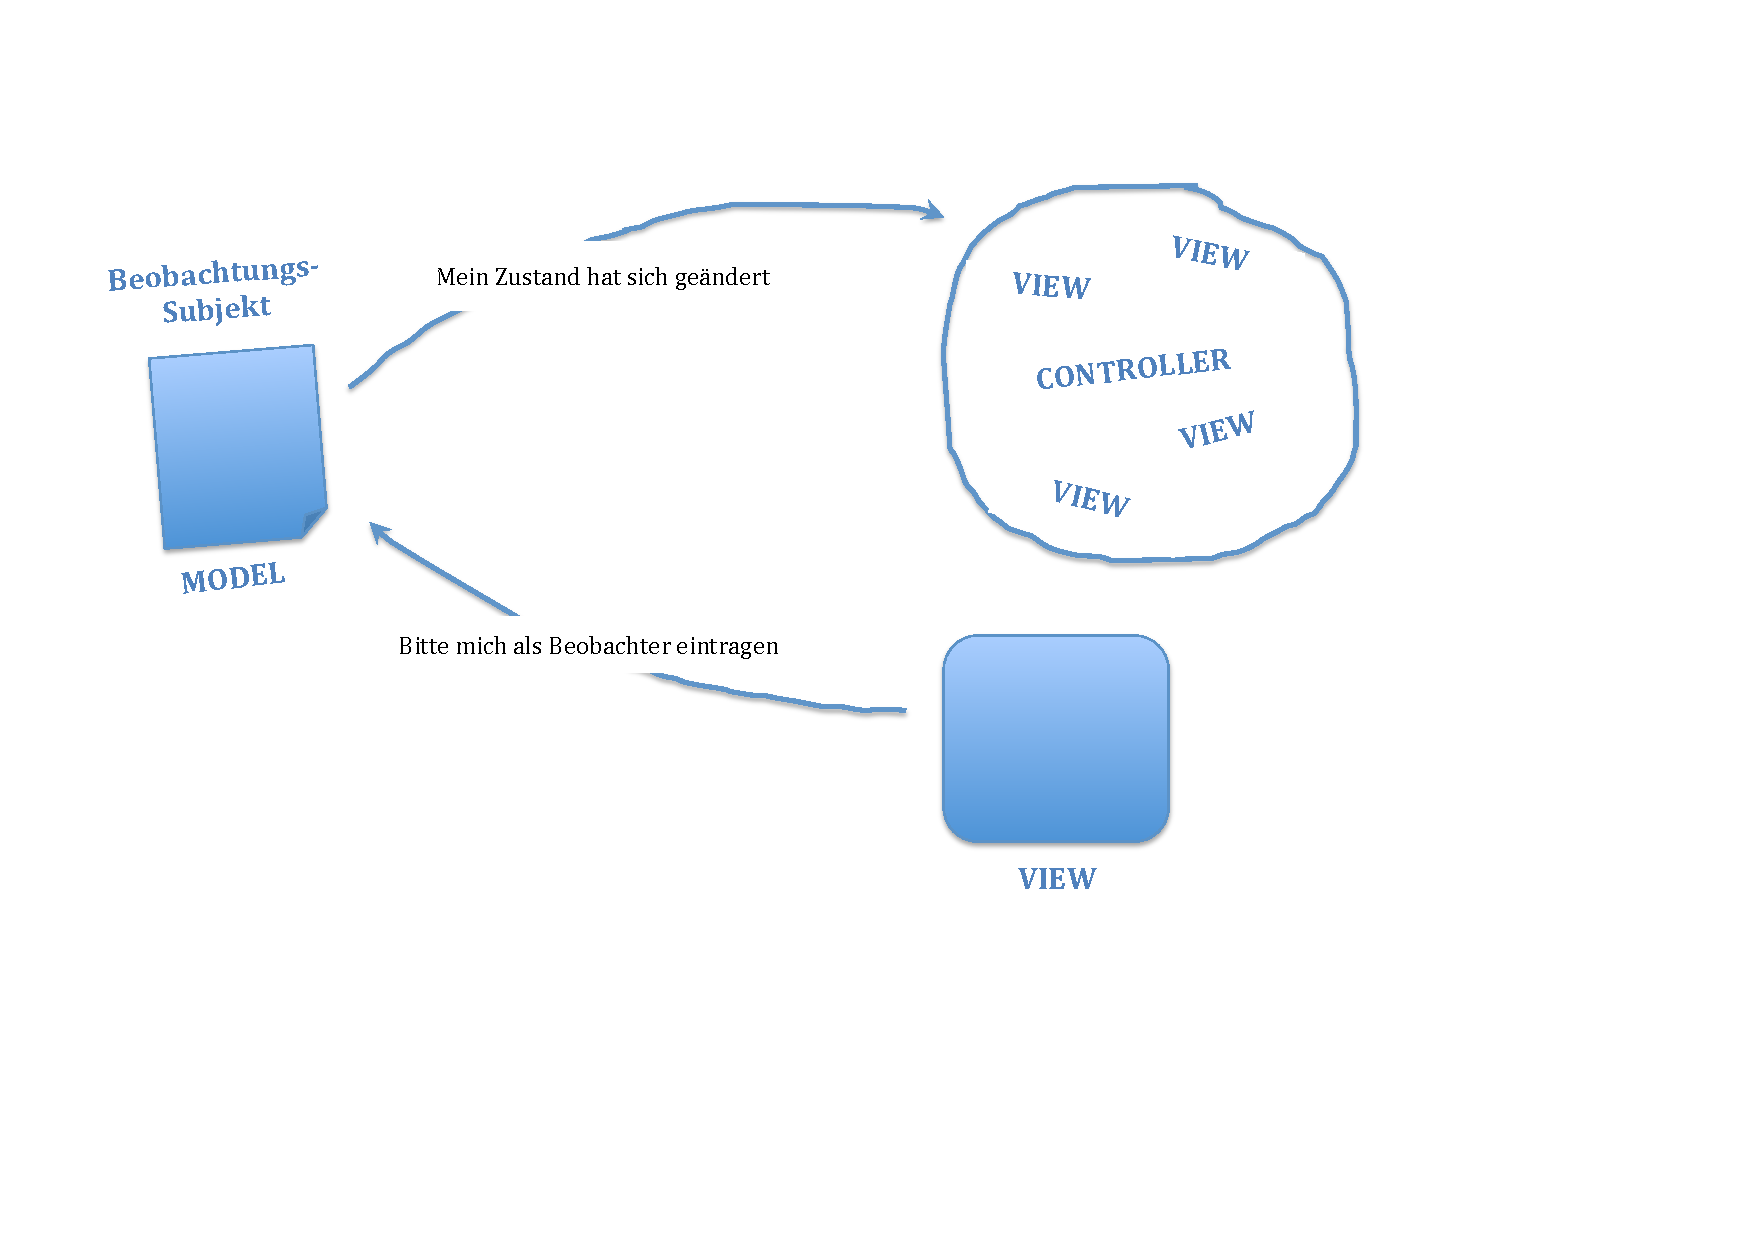
\includegraphics[trim = 0mm 0mm 0mm 0mm, clip, width=0.8\textwidth]{resources/observer}
\caption[Observer Pattern]{Observer Pattern}
\label{img:observer}
\end{figure}

\textbf{Beschreibung des \textbf{Observer}-Pattern Prinzips:}

Die Abbildung \ref{img:observer} zeigt, wie \textbf{Observer}-Pattern im \textbf{MVC} verwendet wird. Wenn ein View bei einer Zustandsänderung des Models informiert werden möchte, registriert er sich beim Model. Der View wird somit in die Liste hinzugefügt, in der sich schon andere Observers befinden können. Im Fall einer Zustandsänderung läuft dann das Model die Liste durch und informiert somit alle, die sich als Beobachter eingetragen haben.
